\documentclass[a4paper,twoside,kulak]{kulakreport}
% LATEX CLASSES
% Standaard: article, report, book, beamer, sciposter
% Huisstijl: kulakarticle, kulakreport, kulakbook, kulakbeamer, kulaksciposter

% PREAMBULE
% dit is het gedeelte tussen \documentclass en de \begin{document}
% hier worden extra pakketten geladen en instellingen gemaakt

% Essentiële pakketten aan het begin van de preambule om correct compileren mogelijk te maken
\usepackage[utf8]{inputenc} % Correct vreemde symbolen inlezen
\usepackage[dutch]{babel}   % Nederlandstalige regels voor woordafbreking
\usepackage[T1]{fontenc}    % Correct vreemde symbolen weergeven

% Instellingen voor titelpagina, kop- en voettekst
% In een standaard article-document zijn er minder mogelijkheden
\faculty{Wetenschap \& Technologie Kulak}
\group{}
\title{Introductie tot \LaTeX}
\subtitle{}
\author{Stijn Rebry}
\emailaddress{stijn.rebry@kuleuven.be}
\institute{KU Leuven Kulak, Wetenschap \& Technologie}
\date{Academiejaar 2018 -- 2019}
\address{
   KU Leuven Kulak           \\
   Wetenschap \& Technologie \\
   Etienne Sabbelaan 53, 8500 Kortrijk             \\
   Tel.\ +32 56 24 60 20     \\
   \href{mailto:\theemailaddress}{\texttt{\theemailaddress}}
   }

% Vaak voorkomende pakketten die aan bod komen in de tekst
\usepackage{amsmath,amssymb,amsthm} % wiskundesymbolen en constructies (American Mathematical Society)
\usepackage{siunitx} % lettertype en spatiëring van fysische eenheden
    \sisetup{decimalsymbol = comma}
\usepackage{epstopdf} % .eps-figuren invoegen 
\usepackage[round]{natbib} % bibliografie in wetenschappelijke stijl
\usepackage{index} % index toevoegen aan het document
\makeindex
\usepackage{cancel} % doorhalingen in formules

% Commando's die worden geïntroduceerd in de tekst
\DeclareMathOperator{\Bgtan}{Bgtan} % lettertype en spatiëring van functies
\DeclareMathOperator{\Bgsin}{Bgsin}
\DeclareMathOperator{\df}{def}
\DeclareMathOperator{\sign}{sign}
\newcommand{\R}{\ensuremath{\mathbb{R}}} % commando zonder argumenten
\newcommand{\C}{\ensuremath{\mathbb{C}}}
\newcommand{\N}{\ensuremath{\mathbb{N}}}
\newcommand{\norm}[1]{\left\|#1\right\|} % commando's met argumenten
\newcommand{\pa}[2]{\frac{\partial #1}{\partial #2}}
\newenvironment{vetmidden}{\begin{center}\bf}{\end{center}} % nieuwe environments
\newtheorem{stelling}{Stelling}[section]
\newtheorem{definitie}[stelling]{Definitie}
\newtheorem*{opmerking}{Opmerking}

% Commando's gebruikt voor het maken van dit document (niet uitgelegd in de tekst)
\newcommand{\code}[1]{\texttt{#1}}
\newcommand{\cmd}[1]{\texttt{\textbackslash#1}\index{commando!#1@\code{#1}}}
\newcommand{\cmdindex}[1]{\index{commando!#1@\code{#1}}}
\newcommand{\opt}[1][]{\texttt{\textbraceleft#1\textbraceright}}
\newcommand{\wis}[1]{\texttt{\textbackslash(#1\textbackslash)}}
\newcommand{\pakket}[1]{\texttt{#1}\index{pakket!#1@\code{#1}}}
\newcommand{\env}[1]{\texttt{#1}\index{omgeving!#1@\code{#1}}}
\newcommand{\klasse}[1]{\texttt{#1}\index{documentklasse!#1@\code{#1}}}

\begin{document} % hier begint de eigenlijke inhoud van het document

\titlepage

\tableofcontents

\chapter{Structuur van een \LaTeX-document}

\section{Preambule en body}

Elk \LaTeX-document\cmdindex{LaTeX} begint met de regel
\begin{verbatim}
\documentclass{...}
\end{verbatim}
waarbij de volledige lay-out van het document bepaald wordt door de naam van een bestaande klasse: \klasse{article}, \klasse{book}, \klasse{beamer}, \klasse{sciposter}, \ldots Dit is meteen het eerste \LaTeX-commando. Deze beginnen steeds met een backslash \code{\textbackslash} en kunnen worden gevolgd door een of meerdere argumenten tussen accolades \code{\textbraceleft\textbraceright}.

De daaropvolgende code is de preambule, waarmee instellingen worden vastgelegd en extra pakketten ingeladen. Onderstaande commando's stellen de titel, auteur en datum van het document in, die weliswaar nog nergens worden afgedrukt maar verderop kunnen worden gebruikt, bijvoorbeeld op het titelblad of in de kop- of voettekst.
\begin{verbatim}
\title{Wiskunde in \LaTeX}
\author{Stijn Rebry}
\date{\today}
\end{verbatim}

Na de preambule volgt de feitelijke inhoud van het document, de  zogenaamde \emph{body}. Deze hoort in de \env{document}-omgeving, dat wil zeggen tussen de commando's \cmd{begin}\opt[document] en \cmd{end}\opt[document]. Het commando \cmd{maketitle} maakt een hoofding op basis van de opgegeven titel, auteur en datum.
\begin{verbatim}
\begin{document}
\maketitle
...
\end{document}
\end{verbatim}

\section{Hoofdstukken}

Een \code{article}-document kent drie kop-niveaus:\cmdindex{section}\cmdindex{subsection}\cmdindex{subsubsection}
\begin{verbatim}
\section{...}
\subsection{...}
\subsubsection{...}
\end{verbatim}
Onmiddellijk na de ontwerpfase van het schrijven, kan de hele structuur van het document dus al met deze commando's worden vastgelegd en in een inhoudstafel gegoten met \cmd{tableofcontents}.

De secties worden automatisch genummerd en geven idealiter elk een duidelijke denkstap uit de tekst weer. Vaste secties zoals inleiding, besluit en inhoudsopgave maken geen deel uit van deze denkstappen en worden derhalve niet genummerd. De nummering kan worden onderdrukt door toevoeging van een asterisk \code{*} aan het kopniveau:\cmdindex{section*}\cmdindex{subsection*}\cmdindex{subsubsection*}
\begin{verbatim}
\section*{...}
\subsection*{...}
\subsubsection*{...}
\end{verbatim}

\section{Omgevingen}

Allerhande soorten structuur en lay-outelementen kunnen worden toegevoegd met behulp van omgevingen, environments:
\begin{verbatim}
\begin{...}
...
\end{...}
\end{verbatim}
Opsommingen (\env{itemize}), genummerde lijsten (\env{enumerate}) en definitielijsten (\env{description}):
\begin{itemize}
\item Een eerste item
\item Nog een item
\item Laatste item
\end{itemize}
\begin{enumerate}
\item Eerste item
\item Tweede item
\item Derde item
\end{enumerate}
\begin{description}
\item[opsommingen] worden in een \env{itemize}-omgeving gezet;
\item[genummerde lijsten] horen in een \env{enumerate}-omgeving;
\item[definitielijsten] maak je met \env{description}, zoals deze.
\end{description}

In bijzondere situaties, bijvoorbeeld brieven, kan het noodzakelijk zijn om zelf met lay-out aan de slag te gaan en van de geijkte paragraafindeling af te wijken: \env{flushleft}, \env{center} en \env{flushright}.
\begin{flushleft}
Links uitgelijnd
\end{flushleft}
\begin{center}
Gecentreerd
\end{center}
\begin{flushright}
Rechts uitgelijnd
\end{flushright}

\section{Bijzondere tekstelementen}

Tekst benadrukken kan met \cmd{emph}\opt\ (\emph{emphasize}). In de klasse \klasse{article} resulteert dit in cursieve tekst (ook te bekomen met \cmd{textit}\opt), maar naargelang de documentklasse kan dat een ander lettertype of kleur zijn. Hoewel het niet altijd te vermijden is, is het de expliciete bedoeling om enkel commando's te gebruiken die structuur te geven aan een document en zo weinig mogelijk commando's die louter lay-out verzorgen. In die zin moet het  verschil tussen de commando's \cmd{emph}\opt\ en \cmd{textit}\opt\ duidelijk zijn: het effect van beide is hetzelfde (in \klasse{article}), maar het tweede commando gaat tegen de geest van \LaTeX\ in.

Voetnoten\footnote{Dit is een voetnoot} kunnen worden ingevoegd met \cmd{footnote}\opt. Met het commando \cmd{marginpar}\opt\marginpar{Een opmerking in de marge} kunnen kernwoorden of opmerkingen in de marge worden gezet.

Stukken programmacode kunnen in doorlopende tekst gezet worden met het \cmd{texttt}-commando. De inhoud van dit commando wordt wel nog door \LaTeX\ als code geïnterpreteerd. Afzonderlijke lijnen met code gaan in een \env{verbatim}-omgeving. In deze omgeving kunnen de meeste \LaTeX-commando's worden weergegeven zonder dat ze worden geïnterpreteerd. Het commando \cmd{verb}\code{|...|} is een bijzonder commando dat speciaal bedoeld is om \LaTeX-commando's te zetten: het schermt alles tussen de symbolen \code{|} af. De weergegeven code mag dus zelf geen symbool \code{|} bevatten, maar wel alle andere \LaTeX-specifieke symbolen zoals een backslash of accolades. Het begin- en eindeteken is echter vrij te kiezen: \cmd{verb}\code{@...@}, \cmd{verb}\code{\%...\%}, \cmd{verb}\code{+...+}, \ldots zolang de voor te stellen code het begrenzend symbool maar niet bevat.

\section{Kruisverwijzingen}
\label{ssec:kruis}

Alle verwijzingen naar hoofdstukken, figuren, vergelijkingen of pagina's moeten altijd automatisch door \LaTeX\ worden gegenereerd, opdat deze automatisch correct zouden zijn en de auteur ze niet handmatig moet opzoeken en corrigeren. 

Hiertoe moet eerst en vooral een onzichtbaar label worden geplaats op de plaats naar waar men wil verwijzen met het \cmd{label}\opt-commando. Met het \cmd{ref}\opt-commando kan dan een referentie naar zo een label worden ingevoerd.  De precieze plaats waar het label staat, bepaalt waarin dit \cmd{ref}\opt-commando wordt vertaald: het nummer \ref{sec:wiskunde} van het volgende hoofdstuk, of van de eerste subsectie \ref{ssec:formules} in dat hoofdstuk of van een welbepaalde formule (\ref{eq:newton}). Een verwijzing naar een ander deel van het document wordt best vergezeld door een paginanummer, met \cmd{pageref}\opt. De paragraaf over kruisverwijzingen start op pagina \pageref{ssec:kruis}

\section{Figuren}

Om figuren in te voegen is het pakket \pakket{graphicx} noodzakelijk -- let op de laatste letter \code{x}, deze is essentieel. Met dit pakket kunnen dan externe \code{.jpg}-, \code{.png}- of \code{.pdf}-bestanden worden ingevoegd. Voor foto's is \code{.jpg} aangewezen. Voor eenvoudigere afbeeldingen zoals screenshots gebruik je best \code{.png}. Vectorafbeeldingen kunnen ingevoegd worden via \code{.pdf}. Programma's die geen \code{.pdf}-exporteermogelijkheden hebben, bieden vaak wel \code{.eps}-figuren aan. Deze kunnen door \LaTeX\ on-the-fly worden geconverteerd naar \code{.pdf} door het pakket \pakket{epstopdf} te gebruiken.

Een figuur wordt ingevoerd met \cmd{includegraphics}\opt. Het argument van dit commando is de bestandsnaam, zonder extensie. De figuur moet zich in dezelfde map bevinden, de extensie moet uit drie kleine letters bestaan en de bestandsnaam moet eenvoudig zijn, zonder vreemde symbolen of spaties, en met respect voor hoofd- en kleine letters worden aangeroepen.

De ingevoegde figuur 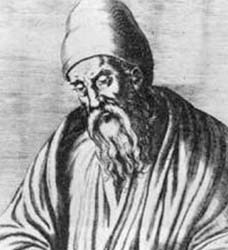
\includegraphics[width=2ex]{euclides} gedraagt zich essentieel als elk ander tekstkarakter. Het kan dus gewoon deel uitmaken van een zin of een paragraaf. De grootte kan worden opgegeven als optioneel argument van de vorm \code{height=5cm} of \code{width=5cm}. Afmetingen in centimeter zijn echter niet te verkiezen. Beter is het gebruik van relatieve maten waardoor de grootte van de figuur zich aanpast naargelang de documentklasse. Twee belangrijke relatieve maten in \LaTeX\ zijn \code{ex}  en \cmd{textwidth}:
\begin{itemize}
    \item \code{2ex} staat voor twee keer de breedte van een letter ``x'',
    \item \code{.5\textbackslash textwidth} neemt de helft van de tekstbreedte in.
\end{itemize}  

Figuren in wetenschappelijke teksten staan meestal echter niet in de doorlopende tekst, maar in een zogenaamde \emph{float} (zie Figuur \ref{fig:euclides} voor een voorbeeld): een zwevende box die op een passende plaats wordt gezet waar zij de bladspiegel het minst stoort en de figuur, een bijschrift en een label bevat. Het bijschrift staat onder de figuur, heeft een nummer, waarnaar minstens één maal vanuit de tekst wordt verwezen middels het label. Dit bijschrift bevat verder een beschrijving van de figuur, zodat de oppervlakkige lezer deze toch kan kaderen. In een langere tekst met veel figuren kan een lijst van figuren worden afgedrukt na de inhoudstafel met het commando \cmd{listoffigures}.

\begin{figure}
\centering
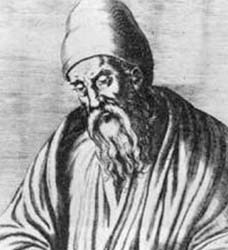
\includegraphics[width=.5\textwidth]{euclides}
\caption{Euclides van Alexandrië}
\label{fig:euclides}
\end{figure}

\section{Tabellen}

Het is mogelijk om in \LaTeX\ eenvoudige tabellen te maken, maar de mark up-taal is minder geschikt voor zeer ingewikkelde tabellen en al helemaal niet voor data-management, daarvoor bestaan andere tools. Tabellen worden gemaakt in een \env{tabular}-omgeving. Deze omgeving heeft als argument de kolomdefinitie: een symbolenrij waarin elke letter staat voor een kolom, naargelang de gewenste uitlijning. De verschillende mogelijk types kolommen en scheidingstekens staan in Tabel \ref{tab:kolommen}.

\begin{table}
\centering
\caption{Kolomtypes en scheidingstekens in tabellen}
\label{tab:kolommen}
\begin{tabular}{l|p{7cm}}
\code{l}    & links uitgelijnde kolom \\
\code{c}    & gecentreerde kolom \\
\code{r}    & rechts uitgelijnde kolom \\
\code{p\textbraceleft7cm\textbraceright} & uitgevulde kolom met opgegeven breedte \newline enkel in dit type kolom kan tekst over verschillende lijnen lopen\\
\code{S} & getallen, gezet zoals met \cmd{num}\opt\ en uitgelijnd op het decimaalteken (pakket \texttt{siunitx})\\
\hline
\code{|}      & verticale lijn tussen twee kolommen \\
\verb|@{...}| & scheidingssymbool tussen twee kolommen
\end{tabular}
\end{table}

In de \env{tabular}-omgeving zelf wordt de inhoud van de tabel rij per rij ingegeven, waarbij de cellen gescheiden worden door een ampersand \code{\&}. Het einde van een rij wordt aangegeven met een dubbele backslash \verb+\\+. Hieronder een tabel met de bijhorende code.

\centerline{
\begin{tabular}{ r || c | l }
	rechts uitgelijnd & gecentreerd & links uitgelijnd \\ \hline
	1                 & 2           & 3
\end{tabular}}

\begin{verbatim}
\begin{tabular}{ r || c | l }
	rechts uitgelijnd & gecentreerd & links uitgelijnd \\
    \hline
	1                 & 2           & 3
\end{tabular}
\end{verbatim}

Net zoals figuren horen grotere tabellen in een \emph{float}. Voor tabellen is er de specifieke omgeving \env{table}. Deze worden ook altijd voorzien van een bijschrift en een label. Het bijschrift staat altijd boven de tabel. In een langere tekst met veel tabellen kan een lijst van tabellen worden afgedrukt na de inhoudstafel met het commando \cmd{listoftables}.


\section{Bibliografie en index}

Het toevoegen van een bibliografie aan een tekst vereist drie elementen: 
\begin{itemize}
    \item Het commando \cmd{bibliographystyle}\opt\ met een argument als \code{plain} of \code{unsrt}. Dit argument bepaalt hoe de citaties zullen worden vormgegeven en gesorteerd. De stijl \pakket{natbib} vereist het gelijknamige pakket en gebruikt vormgeving die in de wetenschappen gebruikelijk is.
    \item Het commando \cmd{bibliography}\opt\ met als argument de naam van een \code{.bib}-bestand dat de bibliografische informatie bevat. Per bron bevat dit bestand een record van de vorm \verb|@book{}| of \verb|@article{}|. De efficiëntste manier om deze bibliografische informatie te verzamelen is ongetwijfeld via \texttt{scholar.google.com}. 
    \item Een citatie met commando \cmd{cite}\opt\ naar een bron uit het \code{.bib}-bestand. In de bibliografie worden enkel die bronnen opgenomen naar dewelke vanuit de tekst expliciet wordt gerefereerd.
\end{itemize}
Om de bibliografie te genereren is het nodig achtereenvolgens de programma's \code{pdflatex}, \code{bibtex}, \code{pdflatex} en opnieuw \code{pdflatex} uit te voeren.

De aangewezen start voor werken met \LaTeX\ is \emph{The Not So Short Introduction to \LaTeXe} \citep{oetiker2010not}. Voor geavanceerder gebruik is een erg uitgebreid naslagwerk \emph{The \LaTeX\ companion} \citep{mittelbach2004latex}.

Het maken van een index vereist het inladen van het pakket \pakket{index} en daaropvolgend het commando \cmd{makeindex}\ in de preambule. Na elk woord waarnaar de index dient te verwijzen, hoort het commando \cmd{index}\opt\ met als argument het lemma. Tot slot staat op de plaats waar de index dient te komen het commando \cmd{printindex}.

\chapter{Wiskunde in \LaTeX}
\label{sec:wiskunde}
\section{Wiskundige symbolen en formules}
\label{ssec:formules}
De functie \(f\) wordt gedefiniëerd als volgt
\[f:\R\to \R:x\mapsto x^2\]
en beeldt een reëel getal \(x\) dus af op het kwadraat \(x^2\). Zowel symbolen als formules horen in \emph{math-mode}, zodat ze allemaal in hetzelfde lettertype worden gezet (cursief in de documentklasse  \texttt{article}. Schrijf dus niet de functie f maar steeds de functie \wis{f}. Naargelang het belang en de grootte van de formule plaats je ze in \emph{inline-style} (zoals het symbool \(f\)) of in \emph{display-style}, op een afzonderlijke regel (zoals de definitie van \(f\)). Wiskundige symbolen als \R\ worden beschikbaar met het pakket \pakket{amssymb}.

Plaats een belangrijke formule in een \env{equation}-omgeving, zo krijgt deze formule een nummer en met label zijn dan kruisverwijzingen mogelijk. Zo stelt de tweede wet van Newton (\ref{eq:newton})
dat kracht \(F\) gelijk is aan massa \(m\) maal versnelling \(a\),
\begin{equation}
\label{eq:newton}
	F=m\cdot a.
\end{equation}

Let er op dat alle symbolen en formules deel uitmaken van een goed gevormde zin. Benoem verder alle symbolen: schrijf niet ``\(F\)'', maar ``de kracht \(F\)'', niet ``\(F=m\cdot a\)'' maar ``de tweede wet van Newton \(F=m\cdot a\)''. Hou volgende vuistregel in gedachten bij het schrijven van een wetenschappelijke tekst die formules bevat: als alle stukken in \emph{math-mode} worden weggelaten, blijft er idealiter een grammaticaal correcte tekst over (die weliswaar niet steeds nog erg zinvol is).

Een berekening loopt vaak over verschillende lijnen. In dat geval is de omgeving \env{align} aangewezen. Deze maakt eigenlijk een \opt[rl] -tabel, waarin je met \code{\&} en \verb|\\| werkt om de invoerregels uit te lijnen. Zonder asterisk worden alle lijnen genummerd, met asterisk krijgen de lijnen in een \env{align*}-omgeving geen nummer. Zo blijken de getallen \(1\) en \(-1\) aan elkaar gelijk te zijn:
\begin{align*}
1 & = \sqrt{1} \\
  & = \sqrt{(-1)\cdot(-1)} \\
  & = \sqrt{(-1)}\cdot\sqrt{(-1)} \\
  & = i\cdot i\\
  & = i^2\\
  & = -1.\\
\end{align*}

\section{Getallen in \LaTeX}

Het zetten van getallen vereist welbepaalde typografische vereisten om de leesbaarheid te maximaliseren. Verschillende manieren om getallen te zetten worden vergeleken in Tabel \ref{tab:getallen}. In principe is het niet nodig om natuurlijke getallen in wiskundemodus te zetten,  de invoer \code{1} en \wis{1} produceren hetzelfde correcte resultaat 1. Voor grote getallen als 1000000000 is het echter gebruikelijk om witruimtes te laten teneinde de leesbaarheid te verhogen, dit manueel doen is nogal bewerkelijk en foutgevoelig. Het teken \code{-} heeft verschillende betekenissen: in tekstmodus is het een koppelteken, invoer \code{-1} heeft foutieve uitvoer -1, in wiskundemodus ziet het er anders uit en is het een minteken, de uitvoer van \wis{-1} is het correcte \(-1\). Het decimaalteken veroorzaakt dan weer een probleem in wiskunde-modus. In principe is het effect 1,1 van de invoer \code{1,1} in tekstmodus correct, maar bij dezelfde code \wis{1,1} in wiskundemodus blijkt de spatiëring na de komma fout: \(1,1\). Dit komt in eerste plaats omdat \LaTeX\ niet een komma maar een punt als decimaalteken gebruikt.

Voor al deze problemen is er één oplossing, namelijk het commando \cmd{num}\opt\ uit het pakket \pakket{siunitx}. Zowel grote \num{1000000000} als negatieve \num{-1} en decimale getallen \num{-1,1} worden automatisch in de correcte lay-out gezet. Voor positieve getallen kleiner dan duizend in tekstmodus en kleine gehele getallen in wiskunde-modus is het commando overkill. Het commando \cmd{num}\opt werkt zowel in tekst- als wiskundemodus en zet voor de uniformiteit ongeacht de invoer overal in het document hetzelfde decimaalteken. In de preambule kan dat desgewenst worden ingesteld als komma: \cmd{sisetup}\opt[decimalsymbol = comma].

Wat in wetenschappelijke teksten vaak voorkomt, zijn tabellen met getallen zoals in Tabel \ref{tab:getallen}. Die worden voor de leesbaarheid zo veel mogelijk op het decimaalteken gealigneerd. Het pakket \pakket{siunitx} voorziet hiertoe de extra kolomdefinitie \code{S}. Deze kolom behandelt alle invoer automatisch net als het \cmd{num}\opt-commando.

\begin{table}
    \centering
    \caption{Verschillende (foute) manieren om getallen te zetten. De juiste gebruikt het commando \cmd{num}\opt\ uit het \texttt{siunitx}-pakket.}
    \label{tab:getallen}
\begin{tabular}{l|l||l|l||l|l}
	  \multicolumn{2}{c||}{Tekstmodus}   & \multicolumn{2}{c||}{Wiskundemodus} &  \multicolumn{2}{c}{\texttt{siunitx}}   \\ \hline
	\texttt{1}       & 1                 & \wis{1}       & $1$                 & \cmd{num}\opt[1]       & \num{1       } \\
	\texttt{-1}      & \xcancel{-1}      & \wis{-1}      & $-1$                & \cmd{num}\opt[-1]      & \num{-1      } \\
	\texttt{1,1}     & 1,1               & \wis{1,1}     & \xcancel{$1,1$}     & \cmd{num}\opt[1,1]     & \num{1,1     } \\
	\texttt{10000}   & \xcancel{10000}   & \wis{10000}   & \xcancel{$10000$}   & \cmd{num}\opt[10000]   & \num{10000  }  \\
	\texttt{0,00001} & \xcancel{0,00001} & \wis{0,00001} & \xcancel{$0,00001$} & \cmd{num}\opt[0,00001] & \num{0,00001 }
\end{tabular}
\end{table}

\begin{table}
    \centering
    \caption{Gealigneerde getallen in een kolom van type \texttt{S}}
    \label{tab:getallen}
    \begin{tabular}{|S|}
    	\hline
    	\text{Dit is tekst} \\
    	123                 \\
    	123456,7            \\
    	-98,76              \\
    	-9.0123456          \\ \hline
    \end{tabular}
\end{table}

\section{Roman of italic?}

Stelt een Latijnse letter een wiskundig object voor, dan staat deze \emph{altijd} cursief. Niet alle Latijnse letters in \emph{math-mode} staan echter cursief. Er zijn een aantal duidelijk afgelijnde uitzonderingen.

Een aaneenschakeling van cursieve symbolen wordt steeds geïnterpreteerd als product van factoren. Bijgevolg stelt \wis{sin x} niet de sinus van \(x\) voor, want het resultaat \(sin x\) dient gelezen als \(s\) maal \(i\) maal \(n\) maal \(x\). Om deze reden worden namen van functies die uit meerdere symbolen bestaan niet cursief gezet: \(\sin x\). Voor courante functies zoals de sinus is er een specifiek commando \cmd{sin}\ met precies dat doel. Niet alle denkbare functies zijn ingebouwd. De boogtangens \(\Bgtan\) bijvoorbeeld, moeten we zelf definiëren, in de preambule met het commando \cmd{DeclareMathOperator}\opt\opt\ uit het pakket \pakket{amsmath}. Het eerste argument is de naam van het te maken \LaTeX-commando en begint dus met een backslash, het tweede argument bevat de naam van de wiskundige functie. Zo een wiskundige operator heeft niet alleen een ander lettertype, maar verzorgt ook de spatiëring tussen de naam van de operator en het argument, en belet dat er tussen beide een regeleinde zou optreden.

Andere uitzonderingen zijn stukjes gewone tekst in een formule, zoals de massa van de aarde \(m_{\text{aarde}}\) of het connectief in volgend verband,
\[\Bgsin(\sin(x))=x \text{ als } x\in [-\frac{\pi}{2},\frac{\pi}{2}].\]
De woorden ``aarde'' en ``als'' zijn geen operatoren maar stukjes gewone tekst die in een grotere formule voorkomen. Plaats dit soort elementen met het commando \cmd{text}\opt.

Een derde situatie waarbij tekst niet cursief in wiskunde-modus staat zijn fysische eenheden, waarvoor het pakket \pakket{siunitx} de commando's \cmd{si}\opt\ en \cmd{SI}\opt\opt\ voorziet. Het eerste zet louter eenheden, het tweede voegt een getal samen met de bijhorende eenheden. De werking van \cmd{SI}\opt\opt\ is weliswaar meer dan het louter aaneenschakelen van commando's \cmd{si}\opt\ en \cmd{num}\opt, het zorgt ook voor spatiëring en belet een lijneinde tussen getal en eenheid.

De valversnelling op Aarde bedraagt \SI{9.81}{m/s^2} en de eenheid van kracht is Newton, en kan uit formule \ref{eq:newton} berekend worden als
\[[\si{N}] = [\si{kg.m/s^2}].\]

\section{Specifieke wiskundige notaties en symbolen}
In het vervolg van de tekst, nog meer dan het voorgaande, gaat vooral om de broncode en veel minder om de tekst zelf. Bestudeer dus eerder de \LaTeX-code dan de resulterende formules.

\[\vec{v}=(v_x,v_y,v_z)\]
%\cmdindex{vec}
%\cmdindex{\_}

\[a^n = \underbrace{a\cdot a\cdot \ldots \cdot a}_{n \text{ keer}}\]
%\cmdindex{^}
%\cmdindex{underbrace}
%\cmdindex{cdot}

\[\lim_{x\to a}f(x)=L\Leftrightarrow \forall \epsilon >0:\exists \delta >0: \forall x\in \df{f}: 0<|x-a|<\delta \Rightarrow |f(x)-L|<\epsilon\]
%\cmdindex{lim}
%\cmdindex{to}
%\cmdindex{Leftrightarrow}
%\cmdindex{forall}
%\cmdindex{epsilon}
%\cmdindex{exists}
%\cmdindex{delta}
%\cmdindex{in}
%\cmdindex{Rightarrow}

\[\frac{df}{dx}(a)=\lim_{x\to a}\frac{f(x)-f(a)}{x-a}\]
%\cmdindex{frac}

\[\int_a^b f(x) dx = \lim_{n\to\infty} \sum_{i=1}^n f(x_i)\frac{b-a}{n} \text{ met } a+(i-1)\frac{b-a}{n}\leq x_i\leq a+i\frac{b-a}{n}\]
%\cmdindex{infty}
%\cmdindex{sum}
%\cmdindex{leq}

\[\det\left[
  \begin{array}{ll}
    a & b\\
    c & d
  \end{array}
  \right]=\left|
  \begin{array}{ll}
  a & b\\
  c & d
  \end{array}
  \right|=ad-bc\]
%\cmdindex{infty}
%\cmdindex{sum}
%\cmdindex{left}
%\cmdindex{right}
%\cmdindex{det}

\begin{equation}
\label{eq:sign}
  \sign : \R\to \{-1,0,1\} : x \mapsto
  \left\{
  \begin{array}{@{}r@{\text{ als }}l}
     1 & x>0\\ 
     0 & x=0\\
    -1 & x<0
  \end{array}
  \right.
\end{equation}


\section{Eigen commando's en omgevingen}

Een zelfgemaakte definitie maak je met \cmd{newcommand}\opt\texttt{[]}\opt. Dit kan handig zijn voor veelvoorkomende symbolen als de getallenverzamelingen \R\ of \C.

Een commando kan tot negen argumenten tellen. Het aantal is een optioneel argument van \cmd{newcommand}\opt\texttt{[]}\opt, het gebruik van deze argumenten kan met \code{\#1} tot \code{\#9}.

\[\norm{\vec{v}},
  \norm{\begin{array}{ll}
    a & b\\
    c & d
  \end{array}}\]
  
\[\pa{f}{x}, \pa{g}{y}, \pa{h}{z}\]

Een eigen omgeving maken kan met \cmd{newenvironment}\opt\opt\opt.

\begin{vetmidden}
Deze tekst is vet en staat gecentreerd.
\end{vetmidden}

Voor definities, stellingen en opmerkingen is het meer specifieke \cmd{newtheorem} uit het \pakket{amsthm}-pakket. Dit maakt genummerde omgevingen zoals de volgende.

\begin{definitie}
Een priemgetal is een natuurlijk getal $p$ dat 
\emph{precies} twee delers in \N\ heeft, namelijk $1$ en $p$.
\end{definitie}

\begin{stelling}[Hoofdstelling van de Getaltheorie]
Elk natuurlijk getal \(a\) verschillend van $0$ en $1$, kan geschreven
worden als product van priemgetallen.
\end{stelling}

\begin{opmerking} Er zijn niet zo veel even priemgetallen, vandaar de legendarische uitspraak: \emph{Two is an odd prime}.
\end{opmerking}

\bibliographystyle{plainnat}
\bibliography{biblio}

\printindex

\end{document}